\documentclass{beamer}
% Définir le thème de la présentation
\usetheme{Madrid}

% Définir le titre et l'auteur de la présentation

\title{Simulateur de Jeu de la Vie}
\author{EL FEJER Marwa\newline DIALLO Mamadou Alpha\newline KOTIN Mahudo Narcisse\newline SOW Mariama Saoudatou}
\institute{Licence 2 informatique}
\titlegraphic{
\includegraphics[width=1cm]{LOGO-UNICAEN.png}}
\subtitle{Chargé de TP: Antonin Callard}
\date{03 mai 2023}

% supprimer la continuation de la frame pour le titre de la section
\setbeamertemplate{frametitle continuation}{}
\AtBeginSection{\frame{\sectionpage}}


\begin{document}

\maketitle
% Table des matières
\begin{frame}
  \frametitle{Table des matières}
  \tableofcontents
\end{frame}

% Section 1
\section{Introduction}



% Slide 1 de la section 1
\begin{frame}
  \frametitle{Introduction}
  
   Le "Jeu de la Vie" est un projet passionnant qui nous a séduit par son potentiel de personnalisation et d'optimisation.\newline 
   
   Ce défi intellectuel nous a permis d'explorer de nouveaux comportements et d'élaborer des solutions innovantes pour résoudre des problèmes complexes.\newline
    
   Au cours de cette présentation, nous vous dévoilerons les fonctionnalités développées et comment elles enrichissent notre simulateur du Jeu de la Vie.

\end{frame}

% Section 2
\section{Fonctionnalités implémentées}

\subsection{Type de voisinage}
\begin{frame}
  \frametitle{Type de voisinage}
 
 \begin{itemize}
 \item Création d'une fonctionnalité pour gérer différents types de voisinage.
 \item Initialement, le voisinage comprend les huit cellules adjacentes.
 \item Configuration personnalisée des voisins pour chaque cellule.
 \item Emploi d'un tableau pour conserver les emplacements relatifs des voisins.
 \item Décompte des voisins vivants en parcourant le tableau et en augmentant un compteur.
 \end{itemize}

\end{frame}

\begin{frame}
  \frametitle{Type de voisinage}
 \begin{figure}
   \centering
   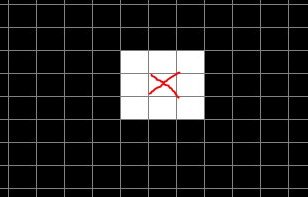
\includegraphics[width=0.7\textwidth]{voisinage_classique.jpeg}
   \caption{Voisinage jeu de la vie classique}
   \label{fig:Type de voisinage}
 \end{figure}
\end{frame}

\begin{frame}
  \frametitle{Type de voisinage}
 \begin{figure}
   \centering
   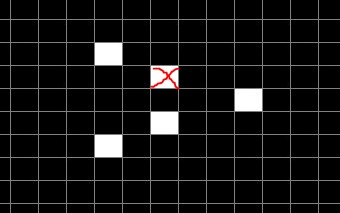
\includegraphics[width=0.7\textwidth]{voisinage_personnalise.jpeg}
   \caption{Voisinage personnalisé}
   \label{fig:Type de voisinage}
 \end{figure}
\end{frame}

% Slide 2 de la section 2
\subsection{Type de règles}
\begin{frame}
  \frametitle{Type de règles}
  
 \begin{itemize}
 \item Personnalisation des règles du jeu.
 \item Utilisation de l'interface "RuleFormat" et classes associées.
 \item Gestion des règles spécifiques avec la classe "Rule".
 \item Vérification de la naissance et survie des cellules.
 \item Validation des règles utilisateur et amélioration de l'efficacité du programme.
 \end{itemize}
 
 
\end{frame}

\begin{frame}
  \frametitle{Type de règles}
 \begin{figure}
   \centering
   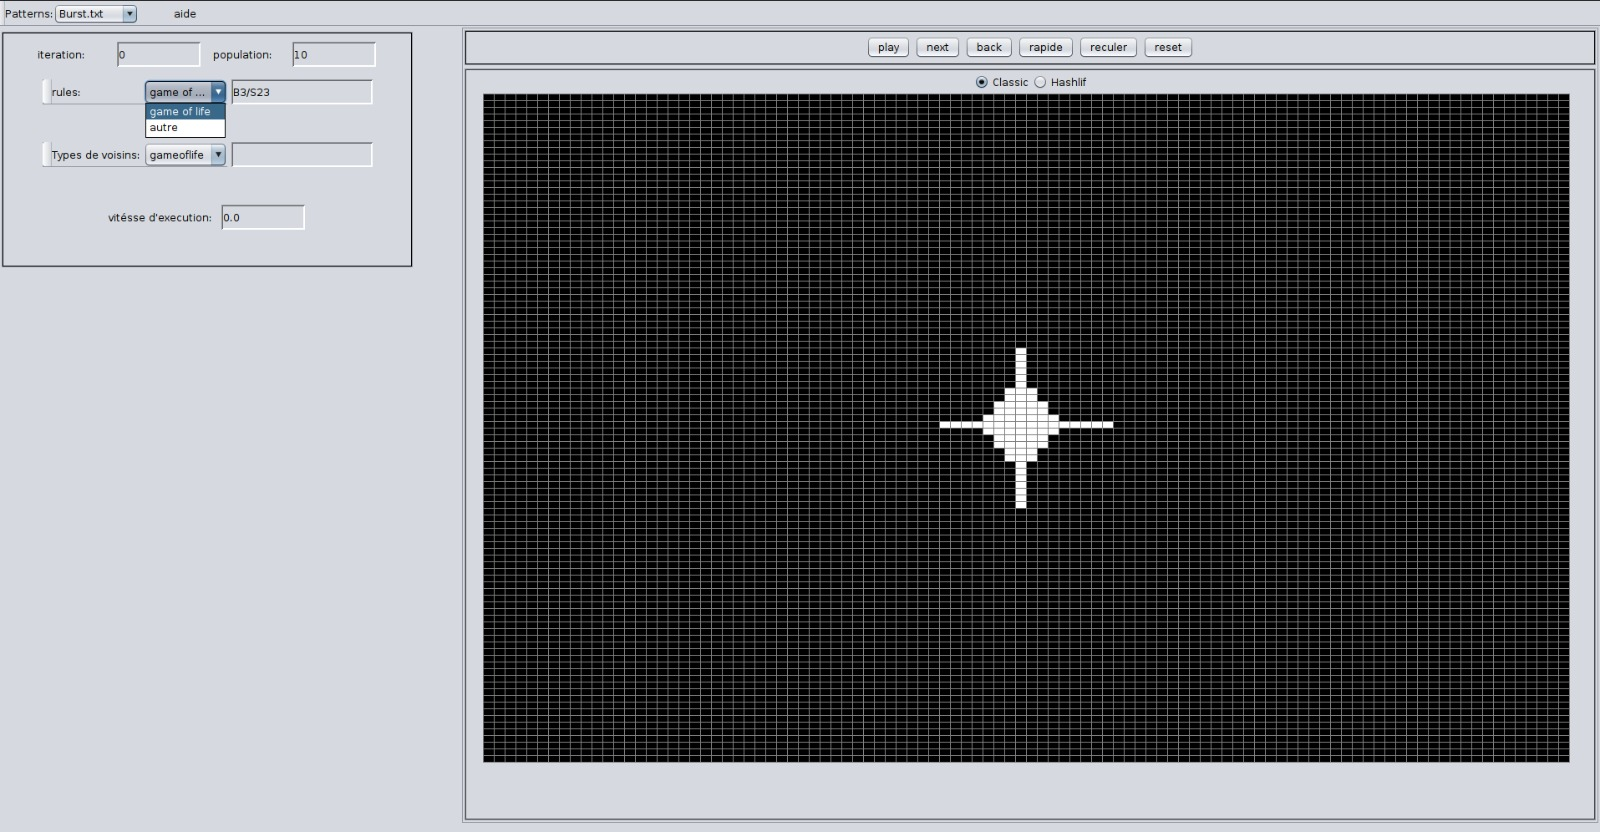
\includegraphics[width=1\textwidth]{image3.jpeg}
   \caption{illustration du bouton rules}
   \label{fig:Type de règles}
 \end{figure}
\end{frame}

% Slide 3 de la section 2
\subsection{Patterns}
\begin{frame}
  \frametitle{Patterns}
 Dans cette partie de la présentation, nous aborderons les points suivants concernant la fonctionnalité d'utilisation des grilles personnalisées :
 
 \begin{itemize}
 \item Initialisation de la grille de jeu avec la méthode "initPattern".
 \item Création et remplissage d'une matrice "pattern".
 \item Vérification des caractères et dimensions de la grille.
 \item Centrage du motif dans la grille de jeu.
 \item Gestion des erreurs et exceptions.
 \end{itemize}
 
\end{frame}

\begin{frame}
  \frametitle{Patterns}
 \begin{figure}
   \centering
   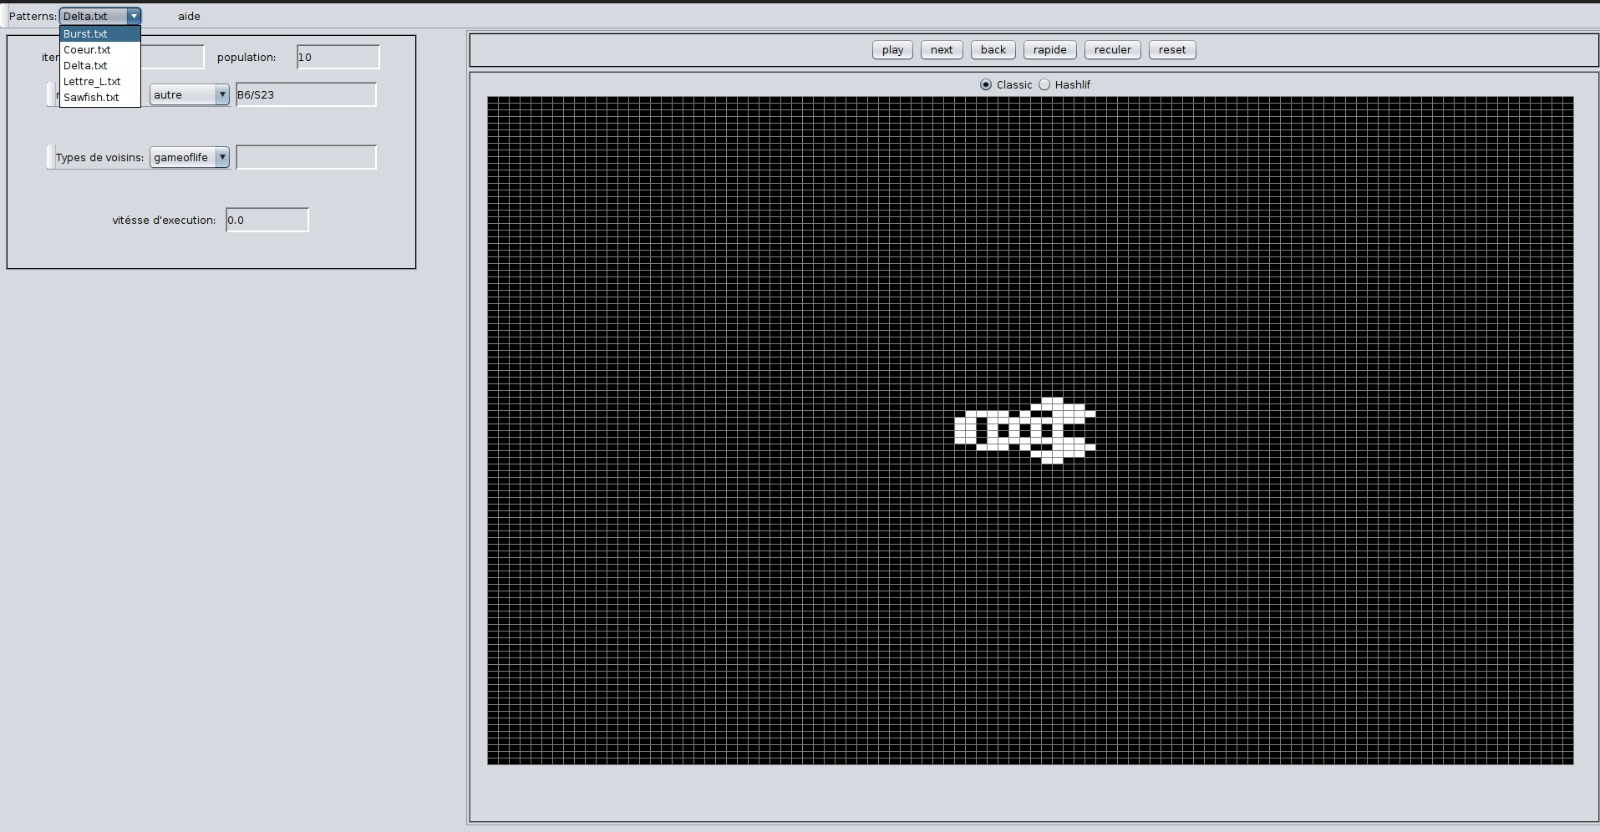
\includegraphics[width=1\textwidth]{image4.jpeg}
   \caption{Exemple d'une image de grille personnalisée}
   \label{fig:patterns}
 \end{figure}
\end{frame}

% Slide 4 de la section 2
\subsection{Algorithme Hashlife}
\begin{frame}
  \frametitle{Algorithme Hashlife}
  
  Dans cette partie nous aborderons les points essentiels pour l'algorithme Hashlife : 
  
 \begin{itemize}
 \item Optimisation du calcul et réduction de l'empreinte mémoire.
 \item Accélération des générations grâce à "jumpGenerations".
 \item Conversion de la grille en quadtree.
 \item Calcul des générations suivantes avec "computeNextGeneration".
 \item Gestion de la vitesse "HashCode" et comparaison d'objets.
 \end{itemize}
\end{frame}

% Slide 5 de la section 2
\subsection{Simulateur}
\begin{frame}
  \frametitle{Simulateur}
 \begin{itemize}
 \item Simulation du jeu de la vie avec un générateur de grilles.
 \item Problème de blocage de l'application pendant la simulation.
 \item Introduction du multi threading pour gérer plusieurs opérations simultanément.
 \item Amélioration des performances grâce au multithreading
 \item Création d'un thread séparé pour le calcul des générations suivantes.
 \item Le thread principal traite les autres opérations simultanément (ex: arrêter la simulation).
 \end{itemize}
\end{frame}

% Démonstration
\section{Démonstration}



% Conclusion
\section{Conclusion}


% Slide de conclusion
\begin{frame}
  \frametitle{Conclusion}
 En conclusion, notre projet sur le Jeu de la vie nous a permis d'approfondir nos compétences en simulation et optimisation, en développant des fonctionnalités pour améliorer la performance et l'expérience utilisateur.\newline
  
 Ce projet passionnant a été une expérience enrichissante, et nous espérons avoir partagé notre enthousiasme avec vous.   

\end{frame}



\end{document}